\documentclass[a4paper, 10pt]{article}

\usepackage[french]{babel}
\usepackage[utf8]{inputenc}
\usepackage[T1]{fontenc}
\usepackage[top=3cm, bottom=3cm, left=3cm, right=3cm]{geometry}
\usepackage{lmodern, amsmath, amssymb, mathrsfs, graphicx, listings, tabularx, color, pgfplots, pgfplotstable, booktabs, titling, authblk, parskip, pgfplots, csquotes, forest, hyperref}
\usepackage[backend=biber, url=false, isbn=false, sorting=none, natbib]{biblatex}
\usepackage[labelfont=sc]{caption}
\usepackage[bottom]{footmisc}

\setlength\parindent{1cm}
\MakeOuterQuote{"}
\hypersetup{colorlinks, linkcolor=black, urlcolor=black}
\pgfplotsset{compat=1.15}
\addbibresource{biblio.bib}
\bibliography{biblio}
\newcommand{\HRule}{\rule{\linewidth}{0.5mm}}
\newcolumntype{Y}{>{\centering\arraybackslash}X}
\newcommand{\Var}{\mathrm{Var}}
\DeclareMathOperator*{\argmax}{arg\,max}


\begin{document}

\begin{titlepage}
\begin{center}
~\\[1cm]
\Large Faculté des Sciences et Ingénierie\\Sorbonne Université\\[3.5cm]
\HRule 
\\[0.4cm]{\huge \bfseries Projet Inpainting :\\[0.1cm] Projet de l'UE Apprentissage et Reconnaissance de Formes\\[0.4cm]}
\HRule \\[1cm] 
\Large \textsc{Julien Denes, Michaël Trazzi} \\[2cm]
\Large Master 1 Informatique, spécialité ANDROIDE\\Année $2017-2018$, Semestre 2 \\[5cm]
\includegraphics[scale=0.3]{logo.png}
\end{center}
\end{titlepage}

\section*{Ressources}

Le présent rapport, les figures qu'ils contient, les sources, ainsi que le code de ce projet, sont disponibles sur Github à l'adresse : \url{https://github.com/mtrazzi/Inpainting}. En particulier, nous avons réalisé des notebook jupyter pour chaque question, disponibles dans le dossier \verb|src| (\url{https://github.com/mtrazzi/Inpainting/tree/master/src}).

\section*{Q1.1 - Régression linéaire, régression ridge et LASSO}

Nous avons ici comparé les algorithmes de regression linéaire, regression ridge et regression lasso en utilisant sklearn.

\subsection*{Ridge}

Afin de déterminer quel était le coefficient de régularisation optimal, nous avons cherché dans le logspace \verb|10**1| à \verb|10**5|. On voit que les coefficients se rapprochent de plus en plus de zéros quand le coefficient de régularisation tend vers l'infini. L'écart-type entre les poids diminue de façon parcimonieuse.

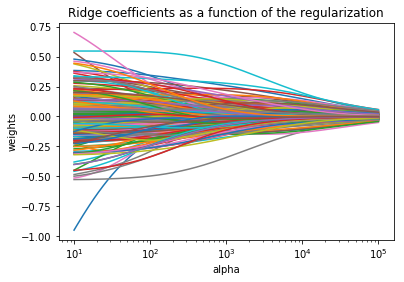
\includegraphics{ridge.png}

La norme du vecteur de poids diminue de façon linéaire (sur l'échelle logarithmique).

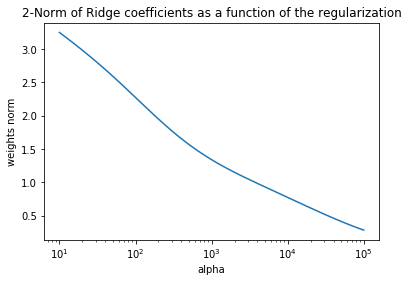
\includegraphics{norm_ridge.png}

\subsection*{Lasso}

Afin de déterminer quel était le coefficient de régularisation optimal, nous avons cherché cette fois-ci dans le logspace \verb|10**-2| à \verb|10**2|. Pour LASSO, les coefficients deviennent tous nuls quand alpha dépasse 1. On voit également que l'écart-type entre poids ne semble pas diminuer. Tout le long, des poids prennent des valeurs extrêmes, pour enfin chuter brusquement vers 0.

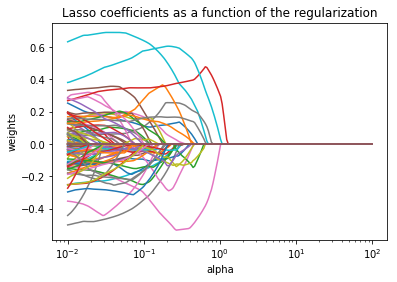
\includegraphics{lasso.png}

La norme du vecteur de poids diminue bien plus brusquement (sur l'échelle logarithmique) pour enfin devenir nul (à partir de alpha = 1).

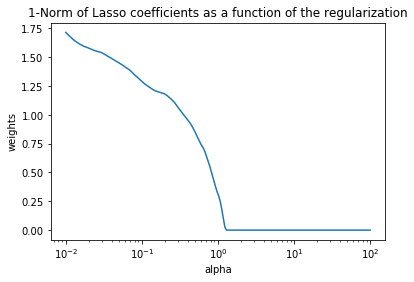
\includegraphics{norm_lasso.png}

\subsection*{Comparaison des algorithmes}

Voici l'écart obtenu entre la prédiction et les labels, sur la base de test des données USPS (entraînement sur la base de données d'entraînement avec les fonctions  \verb|linear_model.RidgeCV| et  \verb|linear_model.LassoCV| afin d'obtenir automatiquement le meilleur coefficient de régularisation (on obtient respectivement $\alpha =142$ et $\alpha =0.005$ pour ridge et lasso)).

\begin{itemize}
    \item Régression linéaire: \verb|MSE| $= 3.7549053135627135$
 \item Ridge: \verb|MSE| $= 3.6942365444755985$ 
\item Lasso: \verb|MSE| $= 3.709303352040891$
\end{itemize}

On voit donc qu'utiliser Lasso ou Ridge n'améliore pas sensiblement la \verb|MSE|. L'intérêt dans ce cas d'utilier Lasso est d'éviter le suraprentissage, en obtenant rapidement un grand nombre de coefficients à 0, à partir de $\alpha = 1$, comme nous avons pu le voir dans les courbes ci-dessus.

\section*{LASSO et inpainting}

On commence pour cette partie par implémentée les fonctions suggérées. En particulier, on peut affichier les images et appliquer un bruitage sur une proportion des pixels :

\begin{centering}
\includegraphics{image1.png}
\end{centering}
\\
\begin{centering}
\includegraphics{image2.png}
\end{centering}

On dispose également de fonctions \texttt{get\_all\_patches}, texttt{get\_bad\_patches} et \texttt{get\_dictionnary} qui permettent respectivement d'obtenir tous les patches possibles, ceux qui comportent du bruitage et le dictionnaire composé de ceux sans bruitage. On trouve par exemple ces éléments respectivement dans chacuns des deux derniers groupes : 

\begin{centering}
\includegraphics{image3.png}
\end{centering}
\\
\begin{centering}
\includegraphics{image4.png}
\end{centering}

Nous avons par la suite souhaité implémenter la méthode d'inpaiting avec Lasso, en utilisant Sklearn. On utilise pour cela le patch à prédire comme label (sous forme de vecteur, auquel on a retiré les pixels noirs) et le dictionnaire comme attributs (sous forme d'un ensemble de $m$ vecteurs, où $m$ est le nombre de patches dans le dictionnaire). On a une unique observation (un seul patch à prédire), puisqu'on ne souhaite pas concevoir un modèle généraliste mais seulement un modèle qui colle parfaitement au patch à prédire. Nos variables d'entrainement sont donc de taille $(1, k)$ pour $Y$, avec $k$ le triple du nombre de pixels dans un patch, et $(1, m, k)$ pour les attributs $X$. En lieu d'attribut, on utilise donc un vecteur du dictionnaire. Le vecteur $w$ que l'on souhaite obtenir devrait donc être de taille $m$.

Nous avons cependant rencontré un blocage lors de la prédiction avec sklearn, puisque ce dernier ne supporte pas les attributs multidimensionnels comme nos vecteurs du dictionnaire. Nous avons donc décidé de transformer $X$ en une matrice de taille $(1, m * k)$. De la sorte, on associe à chaque pixel un poids de chaque pixel de chaque vecteur du dictionnaire. Nous avons ensuite moyenné les poids sur chacun des vecteurs pour obtenir un poids $w$ de taille correcte. Dans les faits, cette méthode se révèle peu efficace puisque tous les poids déterminés par le modèle sont égaux à 0.

La reconstitution des images, possible grâce à la fonction \texttt{recompose}, ne montre donc pas de grands résultats en l'absence de $w$ correct.

\subsubsection*{Partie de l'image manquante}

Lorsqu'on remplit l'image au fur et à mesure des bords vers le centre, l'ordre a une importance. En effet, il suffit de considérer l'exemple d'une photographie d'immeubles sur fond de ciel:

\begin{centering}
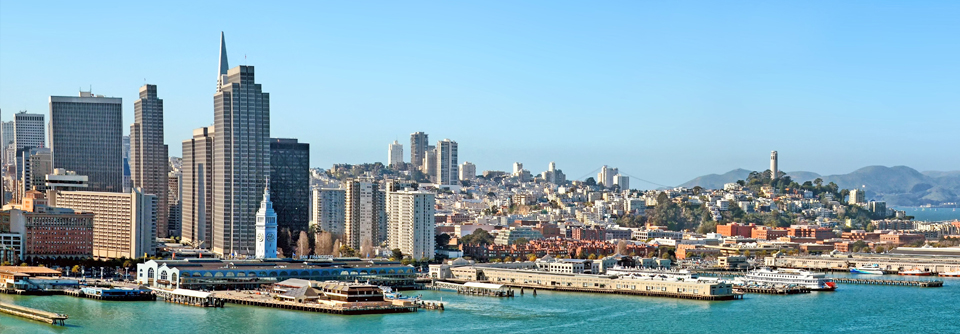
\includegraphics[scale=0.45]{buildings.jpg}
\end{centering}

En parcourant d'abord du haut vers le centre puis du bas vers le centre, l'algorithme va commencer par remplir le haut en ciel car il ne verra pas la base de l'immeuble. En revanche, si on avait commencé en bas, on aurait déjà une base d'immeuble, donc on aurait pu mieux reconstruire le haut de l'immeuble

Plus généralement, on pourra appliquer la technique d'Harrison (P. Harrison. A non-hierarchical procedure for re-synthesis of complex
texture. In Proc. Int. Conf. Central Europe Comp. Graphics, Visua. and
Comp. Vision, Plzen, Czech Republic, February 2001.). C'est la technique utilisée dans "Region Filling and Object Removal by Exemplar-Based Image
Inpainting" : 

\begin{centering}
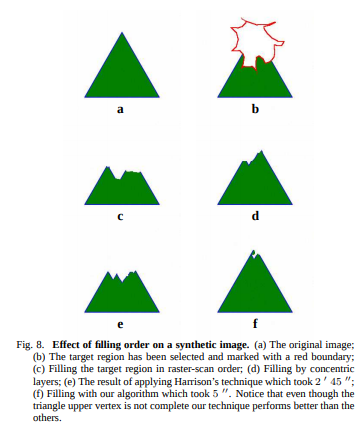
\includegraphics{effects_filling_order.png}
\end{centering}

\end{document}